\documentclass{standalone}
\usepackage{tikz}
\usepackage{verbatim}
\usepackage{xcolor}
\usetikzlibrary{positioning}
\begin{document}
\pagestyle{empty}
  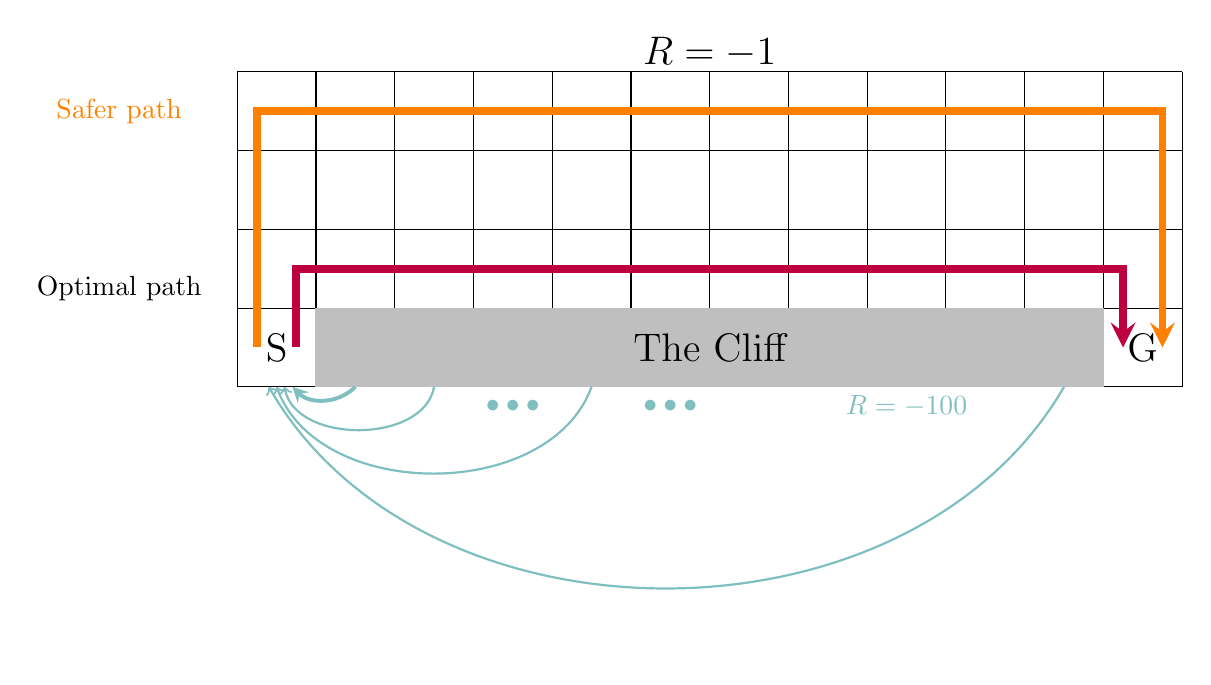
\begin{tikzpicture}
    \draw (0, 0) grid (12, 4);
    \draw[fill,gray!50] (1, 0) rectangle (11, 1);
    \node at (6, 0.5) {\Large The Cliff};
    \node (beg) at (0.5, 0.5) {\Large S};
    \node (end) at (11.5, 0.5) {\Large G};
    \path[draw,purple,thick,-stealth,line width=1 mm] (0.75, 0.5) -- (0.75, 1.5) -- (11.25, 1.5) -- (11.25, 0.5);
    \path[draw,orange,thick,-stealth,line width=1 mm] (0.25, 0.5) -- (0.25, 3.5) -- (11.75, 3.5) --     (11.75, 0.5);
\node at (-1.5, 1.25) {Optimal path};
\node at (-1.5, 3.5)  {\color{orange} Safer path};
\node at (6, 4.25) {\Large $R=-1$};
\path[-stealth,line width=0.5 mm,green!50!blue!50] (1.5,0) edge[bend left=45] (0.7, 0);
\path[->,thick,green!50!blue!50] (2.5,0) edge[bend left=80] (0.6, 0);
\node at (3.5,-0.25) {$\color{green!50!blue!50} \bullet \bullet \bullet$};
\path[->,thick,green!50!blue!50] (4.5,0) edge[bend left=70] (0.5, 0);
\node at (5.5,-0.25) {$\color{green!50!blue!50} \bullet \bullet \bullet$};
\node at (8.5,-0.25) {$\color{green!50!blue!50} R = -100$};
\path[->,thick,green!50!blue!50] (10.5,0) edge[bend left=60] (0.4, 0);
  \end{tikzpicture}
\end{document}